\documentclass[tikz]{standalone}

\usetikzlibrary{arrows, shapes, positioning}

\begin{document}
    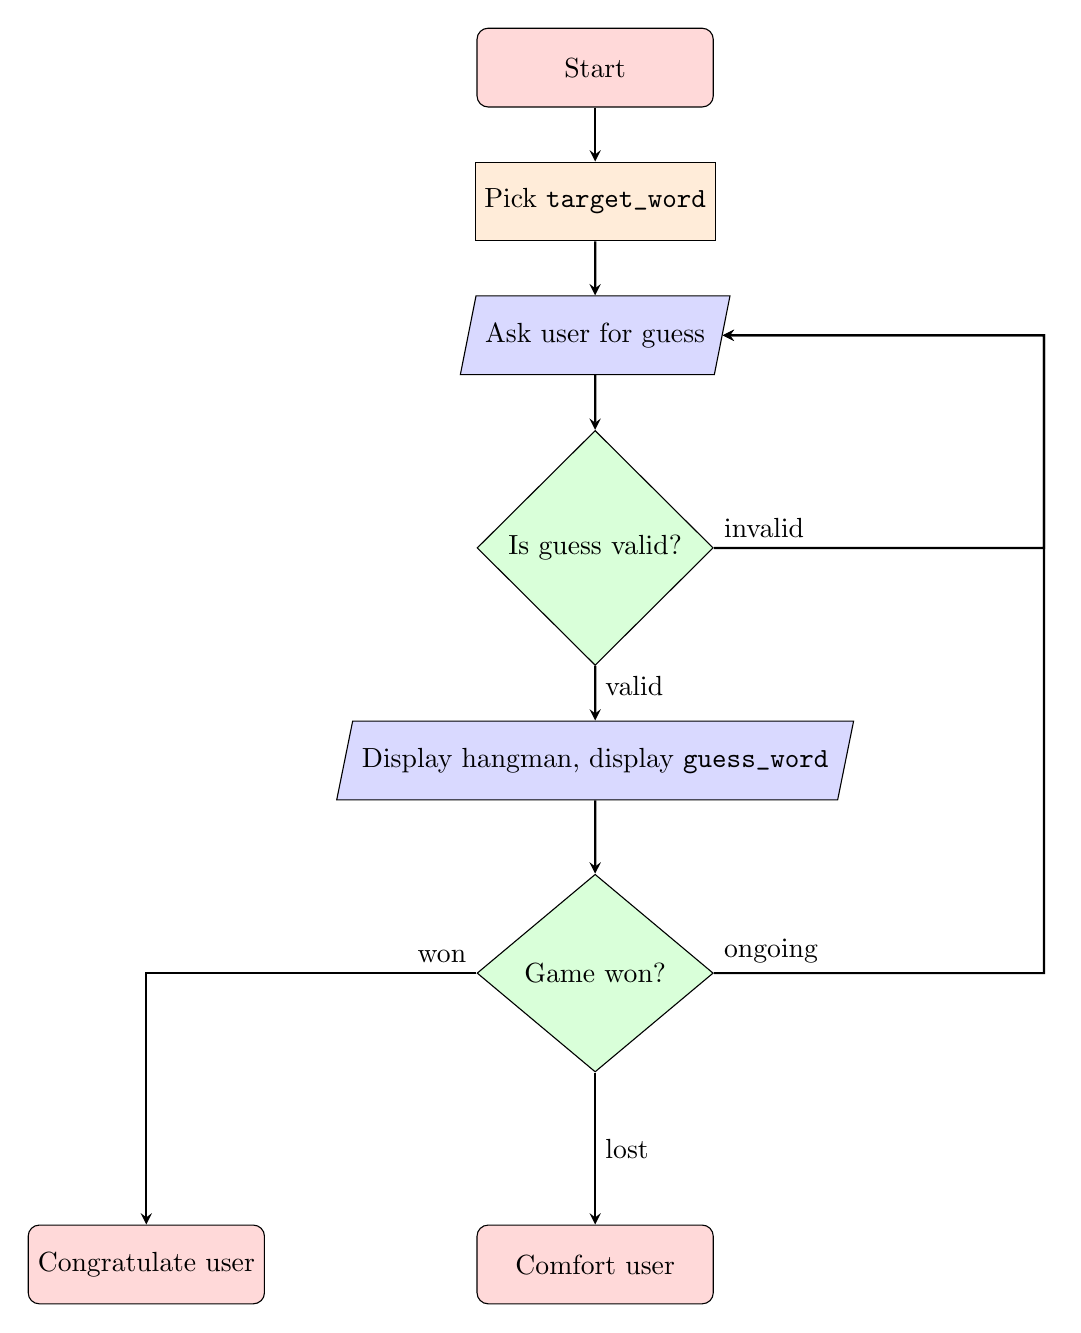
\begin{tikzpicture}[scale=1, node distance=1.7cm]
        \tikzstyle{startstop} = [
    rectangle,
    rounded corners,
    minimum width=3cm,
    minimum height=1cm,
    text centered,
    draw=black,
    fill=red!15
]
\tikzstyle{io} = [
    trapezium,
    trapezium left angle=70,
    trapezium right angle=110,
    minimum width=3cm,
    minimum height=1cm,
    text centered,
    trapezium stretches=true,
    draw=black,
    fill=blue!15
]
\tikzstyle{process} = [
    rectangle,
    minimum width=3cm,
    minimum height=1cm,
    text centered,
    draw=black,
    fill=orange!15
]
\tikzstyle{decision} = [
    diamond,
    minimum width=3cm,
    minimum height=1cm,
    text centered,
    draw=black,
    fill=green!15
]
\tikzstyle{arrow} = [thick, ->, >=stealth]


        \node[startstop] (start) {Start};
        \node[process, below of=start] (random) {Pick \verb|target_word|};
        \node[io, below of=random] (input) {Ask user for guess};
        \node[right of=input, xshift=4cm] (void) {};
        \node[decision, below of=input, yshift=-1cm] (validate) {Is guess valid?};
        \node[io, below of=validate, yshift=-1cm] (display) {Display hangman, display \verb|guess_word|};
        \node[decision, below of=display,  yshift=-1cm] (state) {Game won?};
        \node[startstop, below of=state, yshift=-2cm] (lost) {Comfort user};
        \node[startstop, left of=lost, xshift=-4cm] (won) {Congratulate user};

        \draw[arrow] (start) -- (random);
        \draw[arrow] (random) -- (input);
        \draw[arrow] (input) -- (validate);
        \draw[arrow] (validate.east) node[above right] {invalid} -| (void.center) -- (input.east);
        \draw[arrow] (validate.south) node[below right] {valid} -- (display);
        \draw[arrow] (display) -- (state);
        \draw[arrow] (state.east) node[above right] {ongoing} -| (void.center) -- (input.east);
        \draw[arrow] (state.west) node[above left] {won} -| (won);
        \draw[arrow] (state.south) -- node[right] {lost} (lost);

    \end{tikzpicture}
\end{document}
